
% % This section can go on section:4.2
Mongodb uses the concept of \textit{collections} and \textit{documents} to model data. collections are the grouping of documents which generally have similar schemas. Data in Mongodb has flexible schema where collections do not enforce document structure rather requirements of our application. \todo{A collection is analogous to collection in XML database????}.  Documents are modeled as a data structure following the JSON format which is composed of key and value pair. There are two principle that allow application to represent documents and their relationship: \textit{reference} and \textit{embedded documents}. 
\todo{ need to change following image/json according to xmark data}
\begin{figure}
	\centering
	\subfigure[Reference document]{
		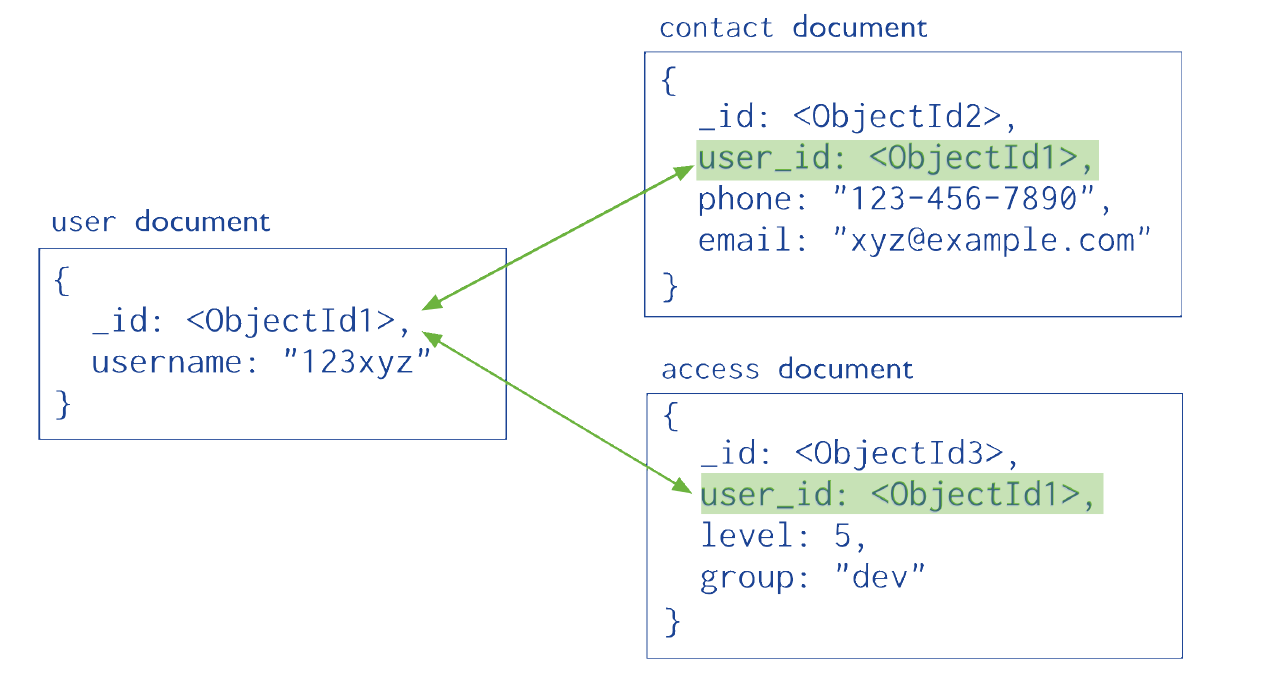
\includegraphics[width=0.44\textwidth]{img/mongodb-reference}
		%\caption{R-tree structure}
		\label{fig:mongodb-ref-doc}
	}
	\centering
	\subfigure[Embedded document]{
		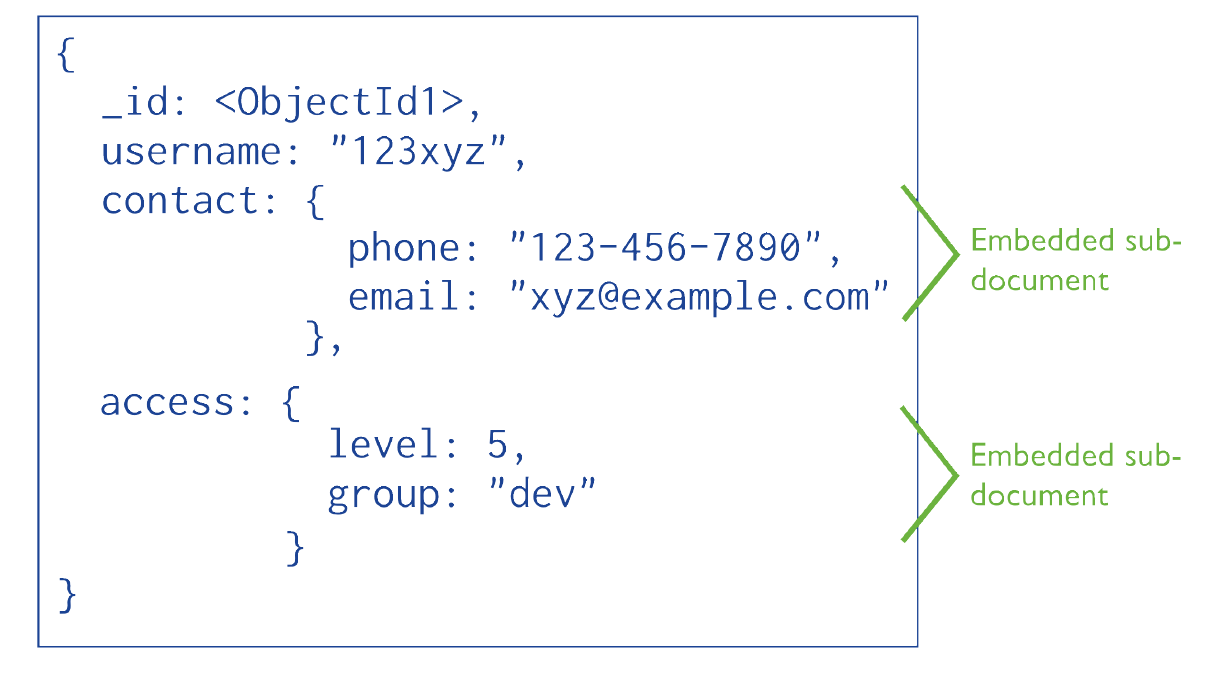
\includegraphics[width=0.44\textwidth]{img/mongodb-embedded}
		%\caption{R-tree}
		\label{fig:mongodb-emb-doc}
	}
	\caption{Mongodb document structure}
	\label{fig:mongodb-doc}
	 
\end{figure}

\paragraph{Reference}
	Reference store the relationships between data by including links and references from one document to another as in  Figure~\ref{fig:mongodb-ref-doc}. The application can resolve these reference to access the related data\todo{Mongodb data model pg4}
\paragraph{Embedded}
	Embedded documents captures relationships between the data by storing related data in a single document structure. The documents in this method are structured as sub-documents\todo{...??} in the in the form of Array or/and Object~\cite{nosql/comparision}. 
	
\paragraph{Indexing} 
	Each document in Mongodb is uniquely identified by a field \textit{\_id} which is a primary index. Hence the collection is sorted by \_id by default. \todo{but note that this primary key index is not a clustered index in Database terms. I.e. the index entries only contains pointers to actual documents in the MongoDB data files. Documents are not physically stored in the order of \_id on disks.??  ::expand...page:9}~\cite{nosql/comparision}
	

\subsubsubsection{XMARK in Mongo}

\begin{fakeJSON}[label=json,caption=Mongodb data representation of XMARk data]
	{
		"_id": "person0",
		"doctype": "people",
		"name": "Kasidit Treweek",
		"emailaddress": "mailto:Treweek@cohera.com",
		"phone": "+0 (645) 43954155",
		"homepage": "http://www.cohera.com/~Treweek",
		"creditcard": "9941 9701 2489 4716",
		"profile": {
			"income": 20186.59,
			"interest": [{
				"category": "category251"
			}],
			"education": "Graduate School",
			"business": "No"
		}
		....
	}
\end{fakeJSON} 

\begin{fakeXML}[label=xml,caption=XMARK data with of \textit{person0}]
	
	<person id="person0">
	<name>Kasidit Treweek</name>
	<emailaddress>mailto:Treweek@cohera.com</emailaddress>
	<phone>+0 (645) 43954155</phone>
	<homepage>http://www.cohera.com/~Treweek</homepage>
	<creditcard>9941 9701 2489 4716</creditcard>
	<profile income="20186.59">
	<interest category="category251" />
	<education>Graduate School</education>
	<business>No</business>
	</profile>
	...
	</person>
\end{fakeXML} 

	
\subsubsubsection{Queries}

	
	
